\documentclass[notheorems,mathserif,table,compress]{beamer}  %dvipdfm选项是关键,否则编译统统通不过
%%------------------------常用宏包------------------------
%%注意, beamer 会默认使用下列宏包: amsthm, graphicx, hyperref, color, xcolor, 等等
\usepackage{fontspec,xunicode,xltxtra}
\usepackage{amsfonts,amssymb}  % for XeTeX
%%------------------------ThemeColorFont------------------------
%% Presentation Themes
% \usetheme[<options>]{<name list>}
\usetheme{Madrid}
%% Inner Themes
% \useinnertheme[<options>]{<name>}
%% Outer Themes
% \useoutertheme[<options>]{<name>}
\useoutertheme{miniframes} 
%% Color Themes 
% \usecolortheme[<options>]{<name list>}
%% Font Themes
% \usefonttheme[<options>]{<name>}
\setbeamertemplate{background canvas}[vertical shading][bottom=white,top=structure.fg!7] %%背景色, 上25%的蓝, 过渡到下白.
\setbeamertemplate{theorems}[numbered]
\setbeamertemplate{navigation symbols}{}   %% 去掉页面下方默认的导航条.
\usepackage{zhfontcfg}
\usepackage{iplouclistings}
\usepackage{fancybox}
\usepackage{latexsym}
\usepackage{xcolor}
\usepackage{multicol}
\usepackage{tabularx}
\usepackage{subfigure} %%图形或表格并排排列
\usepackage{multirow}
\usepackage{tcolorbox}
\newcommand\zhyfly[2][purple]{\hskip5pt\shadowbox{\color{#1}\small\lishu #2\vspace{2mm}}}
\newcommand{\shadow}[2][blue]{\hskip5pt\shadowbox{\color{#1}\small #2\vspace{3mm}}}
%\setsansfont[Mapping=tex-text]{文泉驿正黑}  %% 需要fontspec宏包
     %如果装了Adobe Acrobat,可在font.conf中配置Adobe字体的路径以使用其中文字体
     %也可直接使用系统中的中文字体如SimSun,SimHei,微软雅黑 等
     %原来beamer用的字体是sans family;注意Mapping的大小写,不能写错
     %设置字体时也可以直接用字体名,以下三种方式等同:
     %\setromanfont[BoldFont={黑体}]{宋体}
     %\setromanfont[BoldFont={SimHei}]{SimSun}
     %\setromanfont[BoldFont={"[simhei.ttf]"}]{"[simsun.ttc]"}
%%------------------------MISC------------------------
\graphicspath{{figures/}}         %% 图片路径. 本文的图片都放在这个文件夹里了.
%%------------------------正文------------------------
\begin{document}
\XeTeXlinebreaklocale "zh"         % 表示用中文的断行
\XeTeXlinebreakskip = 0pt plus 1pt % 多一点调整的空间
%%----------------------------------------------------------
%% This is only inserted into the PDF information catalog. Can be left
%% out.
%%%
%% Delete this, if you do not want the table of contents to pop up at
%% the beginning of each subsection:
\AtBeginSection[]{                              % 在每个Section前都会加入的Frame
  \frame<handout:0>{
    \frametitle{内容提要}\small
    \tableofcontents[current,currentsubsection]
  }
}
\AtBeginSubsection[]                            % 在每个子段落之前
{
  \frame<handout:0>                             % handout:0 表示只在手稿中出现
  {
    \frametitle{下一节内容}\small
    \tableofcontents[current,currentsubsection] % 显示在目录中加亮的当前章节
  }
}
%%----------------------------------------------------------
\title[浮游动物图像分类]{基于多特征多分类器组合的海洋浮游动物图像\protect\\分类研究}
%\subtitle{Mathematics of Scientific Computing}
\author[朱亚菲]{姓~~名~~~~~\textcolor{olive}{朱亚菲}\\
    导~~师~~~~~\textcolor{olive}{郑海永}}
\institute[中国海洋大学]{\kaishu\small\textcolor{violet}{中国海洋大学~~信息科学与工程学院}}
\date{2016~年~5~月~22~日}
\titlegraphic{
\includegraphics[height=2cm]{ouc-logo.png}}
%\titlegraphic{\vspace{-6em}\includegraphics[height=7cm]{ouc}\vspace{-6em}}
\frame{ \titlepage }
%%----------------------------------------------------------
\section*{目录}
\frame{\frametitle{目录}\tableofcontents}
%%============================================================================================================================
\section{课题背景}

%-----------------------------------------------------------------------------------------------------------------------------
\begin{frame}
\frametitle{选题背景及意义}
\shadow{浮游动物}
\begin{itemize}
\item 负责浮游植物与高级营养生物之间的能量传递
\item 传输有机物
\item 监测气候变化
\item 干扰水下声纳信号 $\Rightarrow$ 国防军事
\end{itemize}
\begin{figure}
\includegraphics[width=0.6\linewidth]{zooplankton.jpg}
\end{figure}
\end{frame}
%-----------------------------------------------------------------------------------------------------------------------------
\begin{frame}
\frametitle{国内外研究现状}
\begin{displaymath}
\left\{\begin{array}{ll}
\textrm{\color{blue}人工识别}&\\
\textrm{\color{blue}新技术}&\\
\textrm{(光谱法、流式细胞术等)}&\\
\textrm{\color{blue}数字图像处理技术}&\left\{\begin{array}{ll}
\textrm{{\color{red}研究对象:}甲藻、微藻、腰鞭毛虫、}&\\
\textrm{~~~~~~胶州湾浮游动物等}\\
\textrm{{\color{red}特征:}轮廓特征、纹理特征、}\\
\textrm{~~~~~~几何特征、数学形态学特征等}\\
\textrm{{\color{red}分类方法:}决策树、贝叶斯决策、}\\
\textrm{~~~~~~K-最近邻规则、线性判别函数、}\\
\textrm{~~~~~~支持向量机等}\\
\end{array} \right.\\
\end{array} \right.
\end{displaymath}
\end{frame}
%-----------------------------------------------------------------------------------------------------------------------------
\begin{frame}
\frametitle{存在的问题及本文研究思路}
\color{blue}\textbf{存在的问题}
\begin{itemize}
\item 研究对象类别少
\item 采用的特征数目少,没有对大量特征进行有效研究与分析
\item 大多采用单一的分类器
\end{itemize}
\pause
\color{blue}\textbf{研究思路}
\begin{itemize}
\item \textbf{搜集浮游动物图像数据集,对包含{\color{red}多个}类别的浮游动物图像进行研究}
\item \textbf{整理图像处理和计算机视觉领域一些常用的特征,进行{\color{red}特征选择}以挑选出对浮游动物图像分类有效的特征}
\item \textbf{采用{\color{red}分类器融合}的方法提高分类准确率}
\end{itemize}
\end{frame}
%-----------------------------------------------------------------------------------------------------------------------------
\begin{frame}
\frametitle{课题来源}
\begin{enumerate}
\item \rowcolors[]{1}{blue!18}{blue!7}
\begin{tabular}[c]{c|p{6.6cm}}
    项目类别 & 国家自然科学基金\\
    课题名称 & {\heiti 基于视觉注意结合生物形态特征的海洋}\\
              & {\heiti 浮游植物显微图像分析}\\
    课题编号 & 61301240\\
    起止年限 & 2014.01~$\sim$~2016.12\\
  \end{tabular}
  \vspace{5mm}
  \item \rowcolors[]{1}{blue!18}{blue!7}
  \begin{tabular}[c]{c|p{6.6cm}}
    项目类别 & 国家自然科学基金\\
    课题名称 & {\heiti 基于生物形态特征的中国海常见有害赤}\\
              & {\heiti 潮藻显微图像识别}\\
    课题编号 & 61271406\\
    起止年限 & 2013.01~$\sim$~2016.12\\
\end{tabular}
\end{enumerate}
\end{frame}

%============================================================================================================================
\section{浮游动物图像分类基础}
%-----------------------------------------------------------------------------------------------------------------------------
\begin{frame}
\frametitle{实现浮游动物图像分类的基本流程}
\begin{figure}[!htb] %插图
\centering
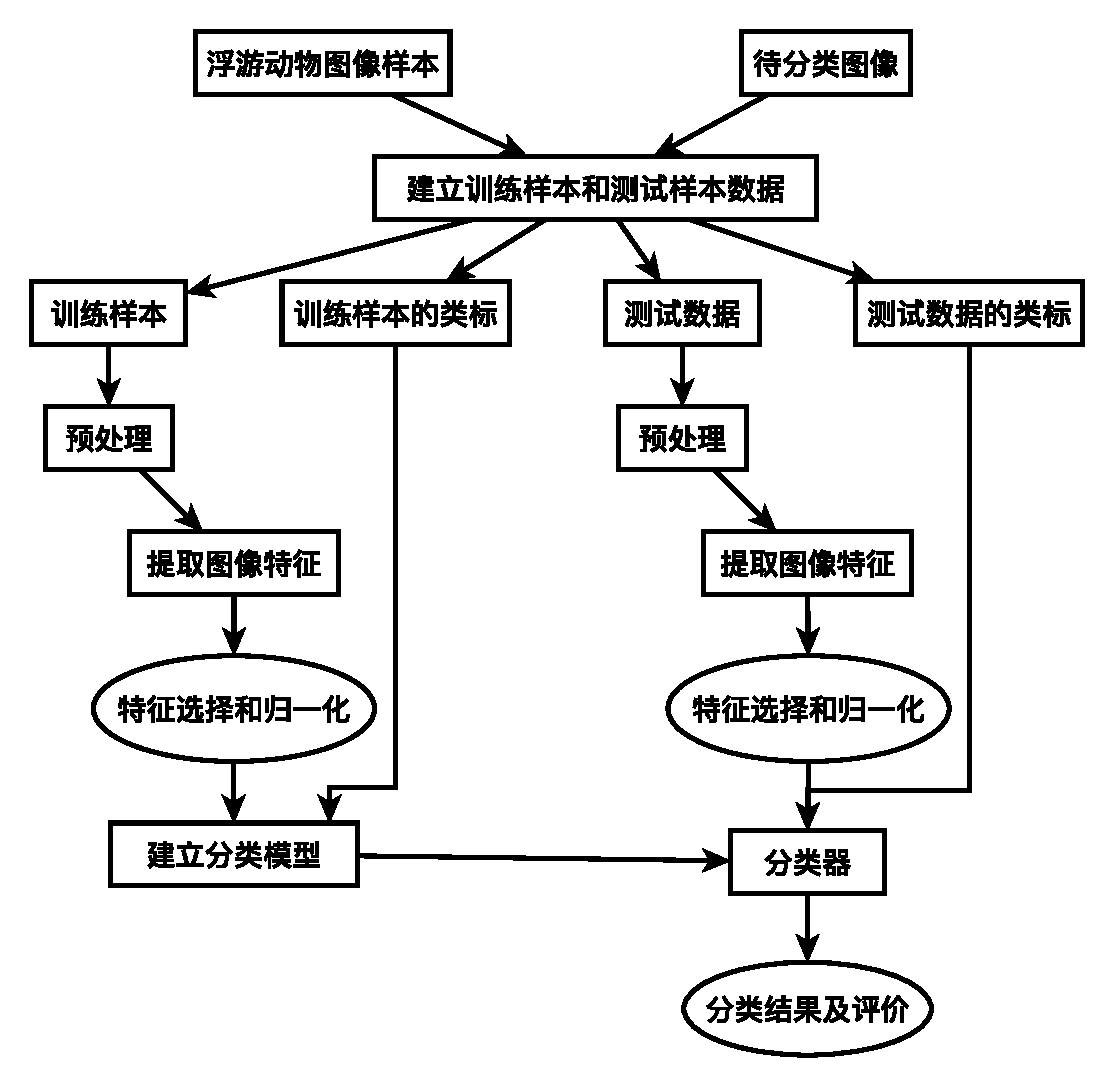
\includegraphics[width=0.6\textwidth]{ClassificationFlowchart.pdf}
\end{figure}
\end{frame}

\subsection{数据集}
%-----------------------------------------------------------------------------------------------------------------------------
\begin{frame}
\frametitle{ZooScan数据集}
\centering
\begin{table}
\small
\rowcolors[]{1}{blue!18}{blue!7}
\begin{tabular}[c]{c|c|c|c}
 & 类别名称 & 训练集图片数目 & 测试集图片数目\\
1 & Appendicularia(尾海鞘纲 )& 545 & 100 \\
2 & Bubble(气泡 )& 145 & 100\\ 
3 & Chaetognatha(毛颚动物门) & 349 & 100\\
4 & Cladocera Penilia(尖头溞属 )& 925 & 100\\
5 & Copepoda(桡脚类) & 1474 & 100\\
6 & Decapoda(十足目) & 557 & 100\\
7 & Doliolida(海樽目) & 285 & 100\\
8 & Egg(卵) & 344 & 100\\
9 & Fiber(纤维 )& 304 & 100\\
10 & Gelatinous(明胶)& 602 & 100\\
11 & Multiple(多个生物)& 635 & 100\\
12 & Pteropoda(翼足目 )& 3078 & 100\\
13 & Nonbio(非生物)& 217 & 100\\
总计 &  & {\color{red}9460} & {\color{red}1300}\\
\end{tabular}
\end{table}
\end{frame}
%-----------------------------------------------------------------------------------------------------------------------------
\begin{frame}
\frametitle{浮游动物图像示例}
\begin{figure}[ht!]
  \subfigure[Appendicularia]{
  \includegraphics[width=0.22\linewidth,height=0.2\linewidth]{Appendicularia.jpg}}
\hspace{0.1in}
\subfigure[Chaetognatha]{
  \includegraphics[width=0.22\linewidth,height=0.2\linewidth]{Chaetognatha.jpg}}
\hspace{0.1in}
\subfigure[CladoceraPenilia]{
  \includegraphics[width=0.22\linewidth,height=0.2\linewidth]{CladoceraPenilia.jpg}}
\\
\subfigure[Doliolida]{
  \includegraphics[width=0.22\linewidth,height=0.2\linewidth]{Doliolida.jpg}}
\hspace{0.1in}
\subfigure[Fiber]{
  \includegraphics[width=0.22\linewidth,height=0.2\linewidth]{Fiber.jpg}}
\hspace{0.1in}
\subfigure[Gelatinous]{
  \includegraphics[width=0.22\linewidth,height=0.2\linewidth]{Gelatinous.jpg}}
 \end{figure}
 \end{frame}

\subsection{评价方法}

%-----------------------------------------------------------------------------------------------------------------------------
\begin{frame}
\frametitle{混淆矩阵}
\begin{center}
\begin{tabular}[c]{|c|c|c|c|}
\hline
 & 类1 & 类2 & 类3\\
 \hline
类1 & 53 & 5 & 2 \\
\hline
类2 & 2 & 55 & 3\\ 
\hline
类3 & 0 & 1 & 59\\ 
\hline
\end{tabular}
\end{center}
\begin{itemize}
\item {真正类率(True Positive Rate, TPR): recall。}
\begin{displaymath}
TPR = \frac{TP}{TP+FN}
\end{displaymath}
\item {伪发现率(False discovery rate, FDR): 1-precision。}
\begin{displaymath}
FDR = \frac{FP}{FP+TP}
\end{displaymath}
\end{itemize}
\end{frame}
%-----------------------------------------------------------------------------------------------------------------------------
\begin{frame}
\frametitle{混淆矩阵}
\begin{multicols}{2}
\shadow{\color{blue}混淆矩阵分类}
~\newline
\begin{itemize}
\item 训练集和测试集相同
\item 训练集和测试集不同(交叉验证)
\end{itemize}
\shadow{\color{blue}交叉验证分类}
~\newline
\begin{itemize}
\item Holdout 验证
\item 留一验证
\item \color{red}K折交叉验证
\end{itemize}
\end{multicols}
\end{frame}

%=============================================================================================================================
\section{浮游动物图像特征提取及分类器设计}

\subsection{特征、分类器选择}
%-----------------------------------------------------------------------------------------------------------------------------
\begin{frame}
\frametitle{特征、分类算法选择}
\shadow{浮游动物图像分类的关键}
\begin{itemize}
\item 特征
\item 分类算法
\end{itemize}
\shadow{特征、分类算法选择的依据}
\begin{itemize}
\item 测试数据集在由该特征和分类算法生成的分类器上的分类准确率达到{\color{red}60\%}以上
\end{itemize}
\end{frame}
%-----------------------------------------------------------------------------------------------------------------------------
\begin{frame}
\frametitle{特征、分类算法整理}
\begin{columns}
\column{.5\textwidth}
\shadow{特征}
\begin{enumerate}
\item ZooScan系统中的67个特征
\item 图像处理领域常用特征
\begin{itemize}
\item 矩形度
\item 体态比
\item 圆形性
\item 偏心率
\item $\cdots$
\end{itemize}
\item 经典特征
\begin{itemize}
\item SIFT
\item HOG
\item LBP
\item 形状上下文 
\item $\cdots$
\end{itemize}
\end{enumerate}
\column{.5\textwidth}
\shadow{分类算法}
\begin{itemize}
\item 支持向量机
\item 随机森林
\item 极限学习机
\end{itemize}
\end{columns}
\end{frame}
%-----------------------------------------------------------------------------------------------------------------------------
\begin{frame}
 \frametitle{特征、分类算法选择结果 }
\begin{tcolorbox}[colback=blue!5,colframe=blue!75!black]
1、从ZooScan系统中选择了对分类有效的22个特征\\
$\Rightarrow$ 随机森林
\end{tcolorbox}
\begin{tcolorbox}[colback=blue!5,colframe=blue!75!black]
2、局部二值模式特征(Local Binary Pattern, LBP)\\
$\Rightarrow$ 支持向量机
\end{tcolorbox}
\begin{tcolorbox}[colback=blue!5,colframe=blue!75!black]
3、内距离形状上下文特征(Inner-Distance Shape Context)\\
$\Rightarrow$ 极限学习机
\end{tcolorbox}
\end{frame}

\subsection{实验}
%-----------------------------------------------------------------------------------------------------------------------------
\begin{frame}
\frametitle{ZooScan系统中的特征}
\centering
{\color{blue}对ZooScan系统中的6类特征用支持向量机和随机森林\protect\\方法进行分类的分类准确率}

~\newline
\rowcolors[]{1}{blue!18}{blue!7}
\begin{tabular}[c]{c|c|c}
& 支持向量机 & 随机森林 \\
位置特征 & 15.3\% & 30.23\% \\
尺寸特征 & 26.04\% & 56.95\% \\
灰度特征 & 37.6\% & 61.3\% \\
形状特征 & 37\% & 63.1\% \\
生物统计特征 & 52.4\% & 69.9\% \\ 
自定义特征 & 68.05\% & 69.03\% \\
\end{tabular}
\end{frame}
%-----------------------------------------------------------------------------------------------------------------------------
\begin{frame}
\frametitle{从ZooScan系统中挑选出的22个特征}
\centering
\rowcolors[]{1}{blue!18}{blue!7}
\begin{tabular}{c|l}
生物统计特征 & 平均值、标准差、灰度直方图偏度、灰度直方图峰度、\\
 & 变异系数、极差偏差 \\
\hline
形状特征 & 分形维数、骨架像素表面积、圆形度、水平对称性、\\
 & 竖直对称性、阈值分割后水平对称性、\\
 & 阈值分割后竖直对称性、延伸率、\\
  & 去掉目标内部空洞的圆形度、包围物体凸包的周长、\\
 & 包围物体凸包的面积\\ 
 \hline
自定义特征 & MeanPos, PerimAreaexc, FeretAreaexc, \\
 & PerimFeret, CDexc \\
\end{tabular}
\end{frame}
%-----------------------------------------------------------------------------------------------------------------------------
\begin{frame}
\frametitle{ZooScan系统的22个特征采用随机森林进行分类的结果}
\begin{figure}[!ht]
\centering
\includegraphics[width=1.0\linewidth,height=2in]{22Features-RF.pdf}
\end{figure}

\centering
\color{red} \fbox{recall = 0.73}
\end{frame}
%-----------------------------------------------------------------------------------------------------------------------------
\begin{frame}
\frametitle{LBP特征采用SVM进行分类的结果}
\begin{figure}[!ht]
\centering
\includegraphics[width=1.0\linewidth,height=2in]{LBP-SVM-2-folds-5-repetitions-32-256.pdf}
\end{figure}

\centering
\color{red} \fbox{recall = 0.64}
\end{frame}
%-----------------------------------------------------------------------------------------------------------------------------
\begin{frame}
\frametitle{内距离形状上下文特征采用ELM进行分类的结果(65张图像作为模板)}
\begin{figure}[!ht]
\centering
\includegraphics[width=1.0\linewidth,height=2in]{IDSC-65-Features-MATLAB-ELM.pdf}
\end{figure}

\centering
\color{red} \fbox{recall = 0.65}
\end{frame}
%=============================================================================================================================
\section{多特征多分类器组合}

\begin{frame}
  \frametitle{多特征多分类器组合方法的基本原理}
\begin{center}
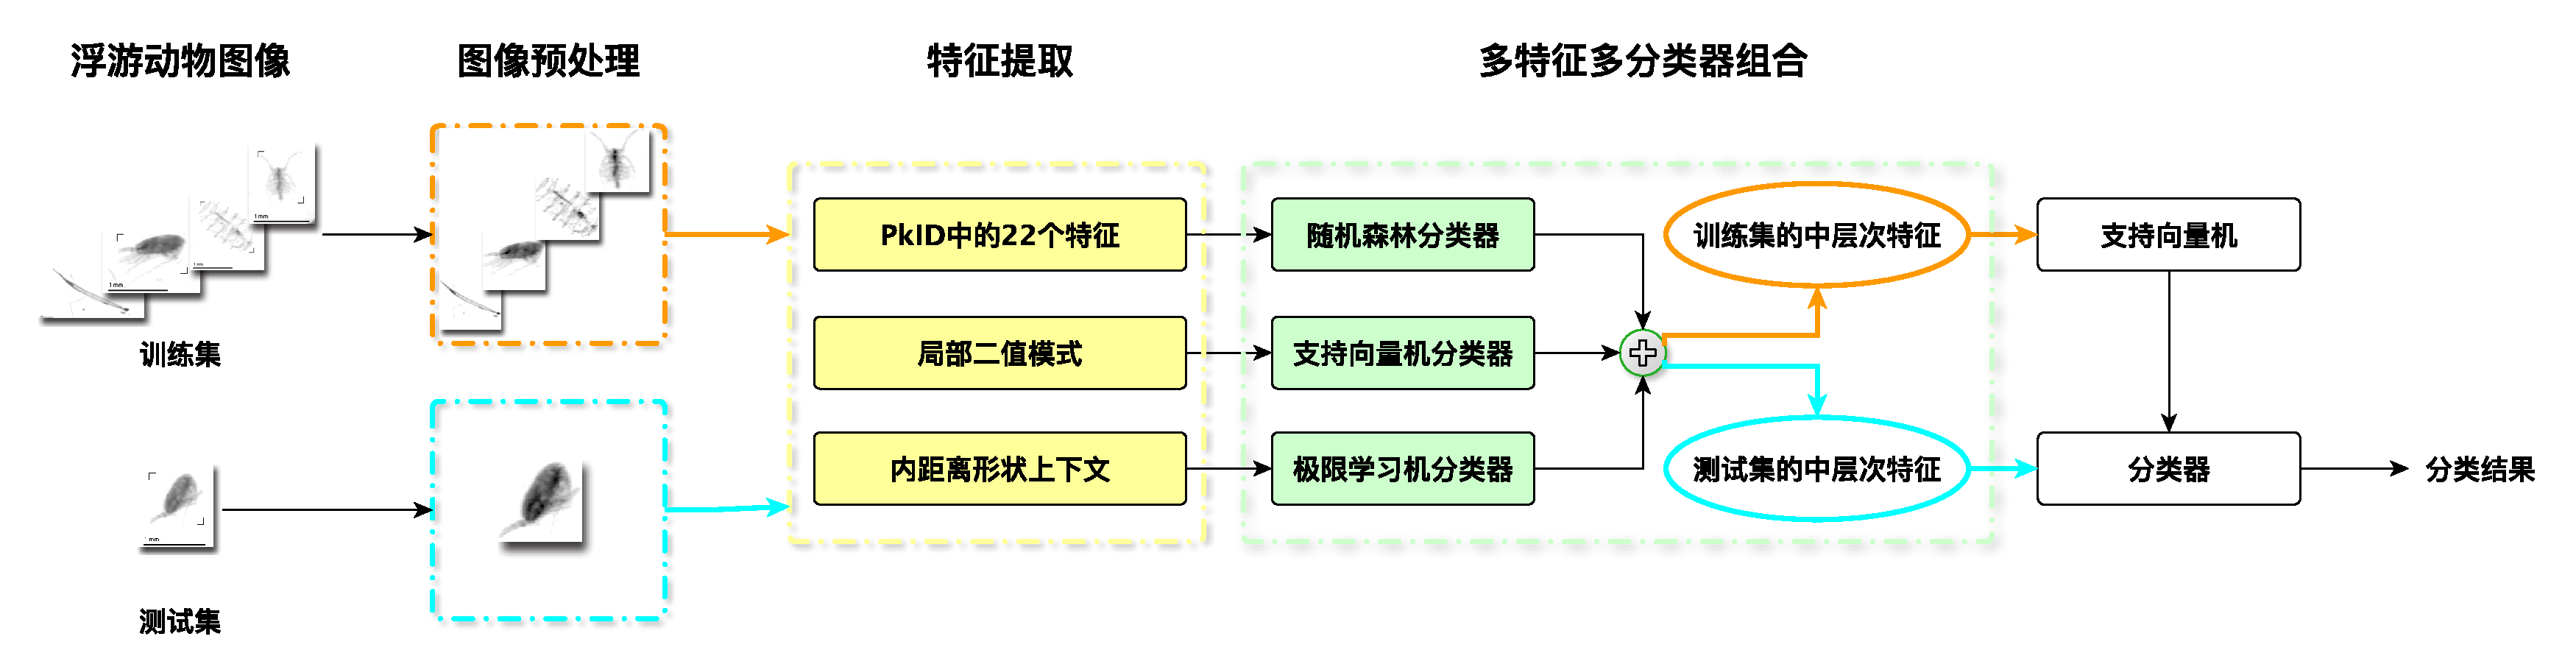
\includegraphics[width=1.0\linewidth,height=1.5in]{framework.pdf}%
\end{center}
\color{red}中层次特征:每幅图像被分到每个浮游动物图像类别的概率($13\times3$维向量)
\end{frame}
%-----------------------------------------------------------------------------------------------------------------------------
\begin{frame}
\frametitle{实验结果对比}
\shadow{\color{blue}ZooScan integrated system}

~\newline
\includegraphics[width=1.0\linewidth,height=2in]{PKID-RF.pdf}

\centering
\color{red} \fbox{recall = 0.75}
\end{frame}
%-----------------------------------------------------------------------------------------------------------------------------
\begin{frame}
\frametitle{实验结果对比}
\shadow{\color{blue}多特征多分类器组合方法}

~\newline
\includegraphics[width=1.0\linewidth,height=2in]{20+IDSC65+LBP-Features-MATLAB.pdf}

\centering
\color{red} \fbox{recall = 0.78}
\end{frame}


%=============================================================================================================================
\section{总结和展望}

%-----------------------------------------------------------------------------------------------------------------------------
\begin{frame}
\frametitle{总结}
\begin{enumerate}
\item 以混淆矩阵中的分类准确率指标作为评价函数,进行特征、分类器的选择。
\item 提出了一种基于多特征多分类器组合的浮游动物图像分类方法。
\end{enumerate}
\end{frame}

%-----------------------------------------------------------------------------------------------------------------------------
\begin{frame}
  \frametitle{展望}
  \begin{enumerate}
\item 针对特征融合进行研究,看看对识别效果的影响。
\item 去除数据集偏见。
  \end{enumerate}
\end{frame}

%=============================================================================================================================
\begin{frame}
\vspace{2cm}

\centering{\color{blue} \kaishu \Huge{ \emph{\textbf{  谢谢!}}}}\\
\vspace{1.5cm}

\begin{flushright}
\emph{\href{mailto:zhuyafei4520@163.com}{\textrm {Yafei~Zhu}}}\\
\href{http://www.ouc.edu.cn}{\textrm {Ocean University of China}}\\
\emph{\textrm {2016.05.22}}
\end{flushright}  
\end{frame}

%%-----------------------------------------------------------------------------------------------------------------------------
%\begin{frame}
%\begin{table}[htbp]
%\fontsize{3pt}{\baselineskip}
%\begin{tabular*}{4cm}{|p{1cm}|c|c|c|c|c|c|c|c|c|c|c|c|c|c|c|c|}
%\hline
% & Appendicularia & Bubble & Chaetognatha & CladoceraPenilia & Copepoda & Decapoda & Doliolida & Egg & Fiber & Gelatinous & Multiple & Nonbio & Pteropoda & Total & Recall & 1-Precision\\
%Appendicularia & 2268 & 0 & 40 & 0 & 4 & 34 & 0 & 0 & 73 & 6 & 79 & 218 & 3 & 2725 & 0.832294 & 0.291693\\
%Bubble & 0 & 202 & 0 & 7 & 6 & 0 & 0 & 364 & 5 & 1 & 1 & 139 & 0 & 725 & 0.278621 & 0.422857\\
%Chaetognatha & 145 & 0 & 1514 & 2 & 1 & 6 & 0 & 1 & 54 & 1 & 7 & 14 & 0 & 1745 & 0.867622 & 0.149916\\ 
%CladoceraPenilia & 0 & 0 & 0 & 3829 & 44 & 31 & 4 & 3 & 0 & 12 & 9 & 692 & 1 & 4625 & 0.827892 & 0.213111\\
%Copepoda & 7 & 0 & 0 & 56 & 5972 & 78 & 5 & 0 & 7 & 27 & 161 & 1053 & 4 & 7370 & 0.810312 & 0.21771\\
%Decapoda & 16 & 0 & 0 & 106 & 115 & 1865 & 1 & 3 & 2 & 22 & 47 & 606 & 2 & 2785 & 0.669659 & 0.231878\\
%Doliolida & 0 & 0 & 0 & 10 & 6 & 0 & 1011 & 4 & 0 & 48 & 23 & 323 & 0 & 1425 & 0.709474 & 0.256071\\
%Egg & 1 & 109 & 0 & 61 & 5 & 13 & 9 & 1136 & 11 & 24 & 11 & 340 & 0 & 1720 & 0.660465 & 0.332158\\
%Fiber & 140 & 0 & 158 & 0 & 9 & 3 & 1 & 5 & 902 & 3 & 101 & 198 & 0 & 1520 & 0.593421 & 0.330861\\
%Gelatinous & 13 & 7 & 0 & 89 & 132 & 11 & 60 & 82 & 7 & 1652 & 101 & 847 & 9 & 3010 & 0.548837 & 0.233766\\
%Multiple & 281 & 0 & 3 & 123 & 367 & 118 & 62 & 10 & 99 & 100 & 537 & 1473 & 2 & 3175 & 0.169134 & 0.632695\\
%Nonbio & 280 & 32 & 56 & 581 & 953 & 261 & 206 & 93 & 186 & 246 & 379 & 12085 & 32 & 15390 & 0.78525 & 0.335989\\
%Pteropoda & 51 & 0 & 10 & 2 & 20 & 8 & 0 & 0 &2 & 14 & 6 & 212 & 760 & 1085 & 0.700461 & 0.065191\\
%Total & 3202 & 350 & 1781 & 4866 & 7634 & 2428 & 1359 & 1701 & 1348 & 2156 & 1462 & 18200 & 813 & 47300 & 0.650265 & 0.285684\\
%\hline
%\end{tabular*}
%\end{table}
%\end{frame}
%
%\begin{frame}
%\begin{tabular}{|l|l|l|l|} 
%\hline  
%\multirow{4}{2cm}{This is a demo table}  
%                & C2a & 
%        \multirow{4}{2cm}{This is another one} & C4a\\ 
%                & C2b &  & C4b\\ 
%                & C2c &  & C4c\\ 
%                & C2d & & C4d\\ 
%        \hline 
%        \end{tabular} 
%\end{frame}


\end{document}
